237. \begin{figure}[ht!]
\center{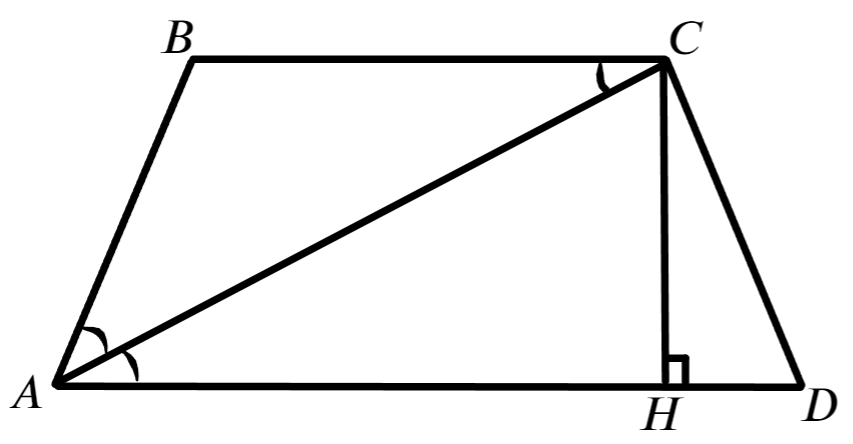
\includegraphics[scale=0.35]{g8-237.png}}
\end{figure}\\
$\angle CAD=\angle ACB$ как накрест лежащие, значит $\angle ACB=\angle BAC$ и треугольник $ABC$ является равнобедренным, поэтому $AB=CD=BC=2$см. Найдём $\angle D=180^\circ-120^\circ=60^\circ,$ тогда $\angle DCH=90^\circ-60^\circ=30^\circ$ ($CH$ --- высота) и по теореме о катете, лежащем напротив угла в $30^\circ,\ HD=CD:2=1$см. Если провести вторую высоту $BH_1,$ то аналогично $AH_1=1$см. Поэтому $P_{ABCD}=2+2+2+1+2+1=10$см.\newpage\noindent
